\documentclass[11pt]{article}

\usepackage{minted,xcolor}
\usemintedstyle{monokai}
\definecolor{bg}{HTML}{282828}
\usepackage{xcolor}
\usepackage{graphicx}
\usepackage{titlesec}
\usepackage[hmargin=2cm,vmargin=2.5cm]{geometry}
\usepackage{fancyhdr}
\usepackage{url}

% \definecolor{line3Color}{HTML}{FFD300}
% \definecolor{line10Color}{HTML}{003688}

\setlength\parindent{0cm}
\setlength\headheight{28pt}

% \titleformat{\section}{\normalfont\huge\bfseries}{Part~\thesection:}{6pt}{}[{\titlerule[0.5pt]}]
% \titleformat{\subsection}{\normalfont\Large\bfseries}{Exercise~\thesubsection:}{6pt}{}

\graphicspath{ {./img/} }

% \title{Practical’s instruction – Networks (week 7)}
% \author{CSC3833 - Data Visualization and Visual Analytic}

\begin{document}

\pagestyle{fancy}
\renewcommand{\headrulewidth}{0pt}
\fancyhead[L]{CSC3833 - Data Visualization and Visual Analytic}
\fancyhead[R]{2023 / 2024}

\begin{center}
\vspace*{1cm}
{\textbf {\Huge Practical Week 7}}\\
\vspace*{0.5cm}
{\textbf {\huge Time Series}}
\vspace*{1cm}
\end{center}

\section{Time Unit}
% -----------------------------------------------------------------------------------------------------

Altair provides a set of tool to interpret and visualize dates. Despite working with various type of data, it works better using \textit{NumPy} \textit{datetime64} and \textit{timedelta64} data types. You can transform your data using the function \textit{to\_datetime} of the \textit{pandas} library.\\
\\
Let's work with a dataset already in the \textit{datetime64} format, containing hourly temperatures measured in Seattle.

\begin{minted}[bgcolor=bg, frame=lines, framesep=2mm]{python}
import altair as alt
from vega_datasets import data

# Disable the maxumin number of row to be able to dispay such large datatset
alt.data_transformers.disable_max_rows()

temps = temps = data.seattle_temps()
temps.head()
\end{minted}

Now display the dataset.

\begin{minted}[bgcolor=bg, frame=lines, framesep=2mm]{python}
alt.Chart(temps).mark_line().encode(
    x='date:T',
    y='temp:Q'
)
\end{minted}

\begin{center}
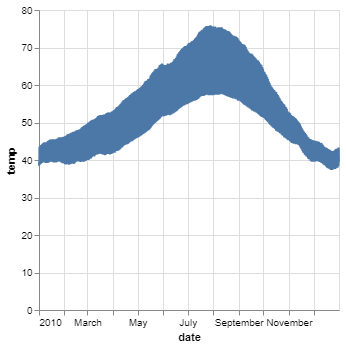
\includegraphics[width=.5\textwidth]{visualization (1).png}
\end{center}

Notice that for date/time values we use the \textit{T} to indicate a temporal encoding: while this is optional for \textit{NumPy} datetime input, it is good practice to specify a type explicitly.\\
\\
For date-time inputs like these, it can sometimes be useful to extract particular time units (e.g. hours of the day, dates of the month, etc.). In Altair, this can be done with the following time unit transforms:

\begin{itemize}
    \item "year", "yearquarter", "yearquartermonth", "yearmonth", "yearmonthdate", "yearmonthdatehours", "yearmonthdatehoursminutes", "yearmonthdatehoursminutesseconds"
    \item "quarter", "quartermonth"
    \item "month", "monthdate"
    \item "date" (Day of month, i.e., 1 - 31)
    \item "day" (Day of week, i.e., Monday - Friday)
    \item "hours", "hoursminutes", "hoursminutesseconds"
    \item "minutes", "minutesseconds"
    \item "seconds", "secondsmilliseconds"
    \item "milliseconds"
\end{itemize}

Let's plot only the mean monthly temperature.

\begin{minted}[bgcolor=bg, frame=lines, framesep=2mm]{python}
alt.Chart(temps).mark_line().encode(
    x='month(date):T',
    y='mean(temp):Q'
)
\end{minted}

\begin{center}
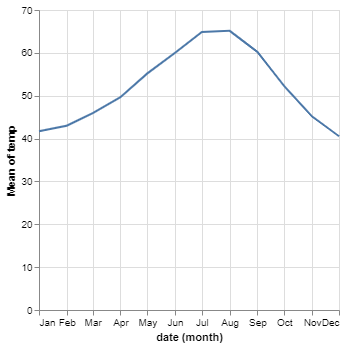
\includegraphics[width=.5\textwidth]{visualization (2).png}
\end{center}

Notice that by default time unit output is a continuous quantity; if you would instead like it to be a categorical, you can specify the ordinal (O) or nominal (N) type. This can be useful when plotting a bar chart or other discrete chart type:

\begin{minted}[bgcolor=bg, frame=lines, framesep=2mm]{python}
alt.Chart(temps).mark_bar().encode(
    x='month(date):O',
    y='mean(temp):Q'
)
\end{minted}

\begin{center}
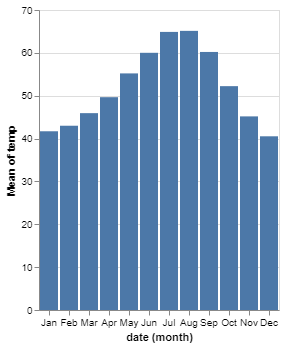
\includegraphics[width=.5\textwidth]{visualization (3).png}
\end{center}

Multiple time units can be combined within a single plot to yield interesting views of your data; for example, here we extract both the hour of the day and the day of the month to give a profile of Seattle temperatures through the year.\\
\\
For clarity in this example, we'll limit ourselves to the first two weeks of data.

\begin{minted}[bgcolor=bg, frame=lines, framesep=2mm]{python}
temps = temps[temps.date < '2010-01-15']

alt.Chart(temps).mark_rect().encode(
    alt.X('hoursminutes(date):O').title('hour of day'),
    alt.Y('monthdate(date):O').title('date'),
    alt.Color('temp:Q').title('temperature (F)')
)
\end{minted}

\begin{center}
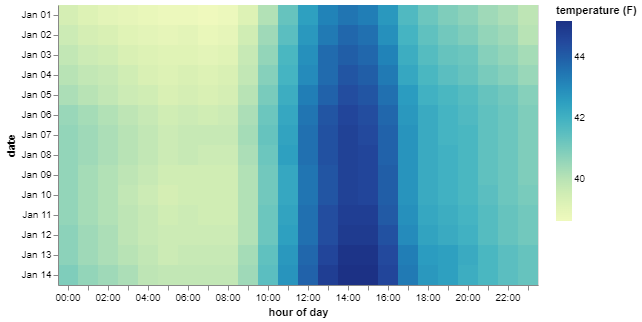
\includegraphics[width=.7\textwidth]{visualization (4).png}
\end{center}

\section{Specifying Time Zones}
% -----------------------------------------------------------------------------------------------------

In the previous example the times are both serialized and rendered in local time, so that the January 1st 00:00:00 row renders in the chart as 00:00 on January 1st.\\
\\
In Altair, simple dates without an explicit timezone are treated as local time. If you would like your dates to be time-zone aware, you can set the timezone explicitly in the input dataframe. Since Seattle is in the US/Pacific timezone, we can localize the timestamps in Pandas as follows:

\begin{minted}[bgcolor=bg, frame=lines, framesep=2mm]{python}
temps['date_pacific'] = temps['date'].dt.tz_localize('US/Pacific')
\end{minted}

Notice that the timezone is now part of the pandas datatype. If we repeat the above chart with this timezone-aware data, the result will render according to the timezone of the browser rendering it:

\begin{minted}[bgcolor=bg, frame=lines, framesep=2mm]{python}
alt.Chart(temps).mark_rect().encode(
    alt.X('hoursminutes(date_pacific):O').title('hour of day'),
    alt.Y('monthdate(date_pacific):O').title('date'),
    alt.Color('temp:Q').title('temperature (F)')
)
\end{minted}

\begin{center}
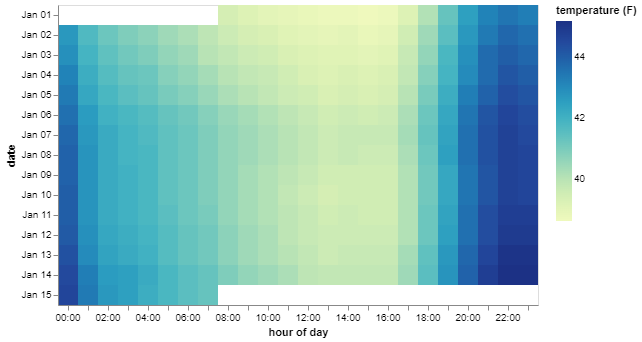
\includegraphics[width=.7\textwidth]{visualization (5).png}
\end{center}

If you are viewing this chart on a computer whose time is set to the west coast of the US, it should appear identical to the first version. If you are rendering the chart in any other timezone, it will render using a timezone correction computed from the location set in your system.

\section{Using UTC Time}
% -----------------------------------------------------------------------------------------------------

This user-local rendering can sometimes be confusing, because it leads to the same output being visualized differently by different users. If you want timezone-aware data to appear the same to every user regardless of location, the best approach is to adopt a standard timezone in which to render the data. One commonly-used standard is Coordinated Universal Time (UTC). In Altair, any of the time unit bins can be prefixed with utc in order to extract UTC time units.\\
\\
Here is the above chart visualized in UTC time, which will render the same way regardless of the system location:

\begin{minted}[bgcolor=bg, frame=lines, framesep=2mm]{python}
alt.Chart(temps).mark_rect().encode(
    alt.X('utchoursminutes(date_pacific):O').title('UTC hour of day'),
    alt.Y('utcmonthdate(date_pacific):O').title('UTC date'),
    alt.Color('temp:Q').title('temperature (F)')
)
\end{minted}

\begin{center}
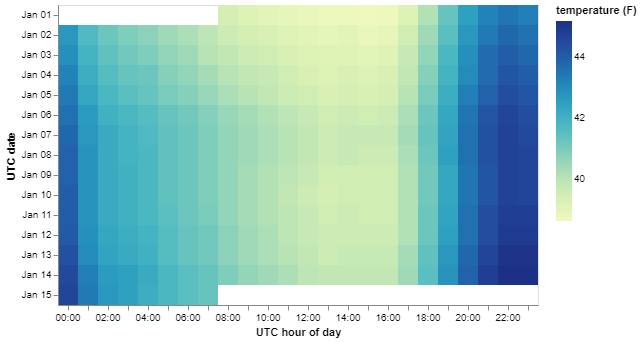
\includegraphics[width=.7\textwidth]{visualization (6).png}
\end{center}

\section{Horizon Chart}
% -----------------------------------------------------------------------------------------------------

Based on what you've learned so far, and using external sources, create an horizon chart of the highest temperatures in Seattle for each month of an entire year.\\
\\
Tips:
\begin{itemize}
    \item Use the \textit{row} parameter of the \textit{encode} function to create multiple views.
    \itme Remove zero as the minimum value of the scale for the scale for more readability.
\end{itemize}

\subsubsection*{Expected result}

\begin{center}
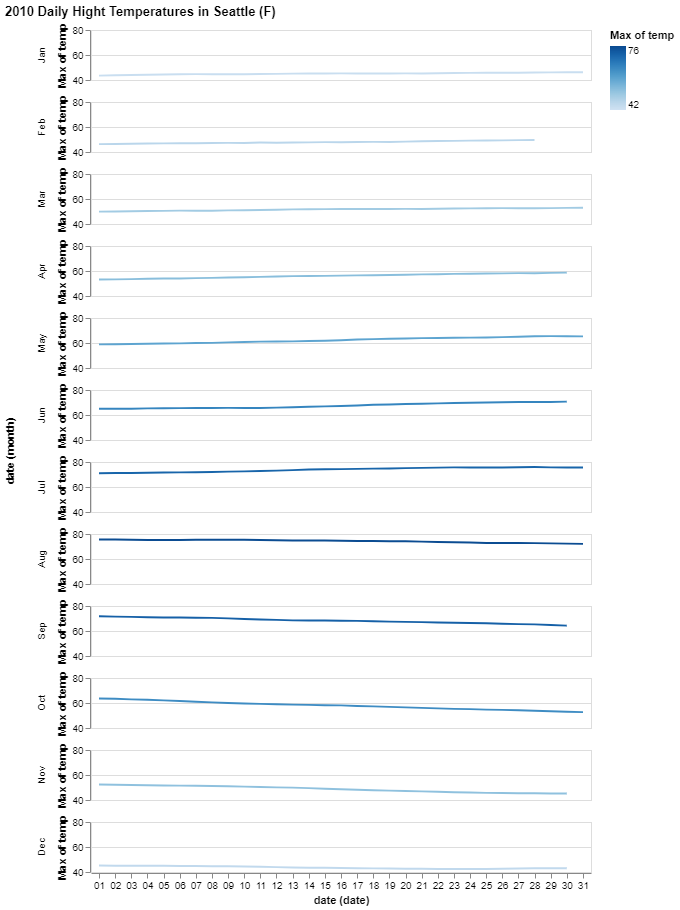
\includegraphics[width=.7\textwidth]{visualization (7).png}
\end{center}

\subsection*{Solution}

\begin{minted}[bgcolor=bg, frame=lines, framesep=2mm]{python}
# Reload the data to access a full year
temps = data.seattle_temps()
temps = temps[temps.date < '2010-12-31']

chart = (
    alt.Chart(temps)
    .mark_line()
    .encode(
        alt.X('date(date):O'),
        # Remove zero as the minumum value of the scale to access further detail
        alt.Y('max(temp):Q').scale(zero=False),
        alt.Color('max(temp):Q'),
        row='month(date):O'
    )
    .properties(
        width=500,
        height=50,
        title="2010 Daily Hight Temperatures in Seattle (F)"
    )
)

chart
\end{minted}

\section{Financial Data}
% -----------------------------------------------------------------------------------------------------

Most low latency real time sources of market data require paid for subscriptions, but it is possible to retrieve large amounts of data for free. One is a library called \textit{yfinance} accessing market data published by \textit{Yahoo}.\\
\\
Start by installing such library.

\begin{minted}[bgcolor=bg, frame=lines, framesep=2mm]{python}
pip install yfinance
\end{minted}

Now load \textit{Unilever} data for 2022. \textit{Unilever} standard ticker is 'ULVR.L'.

\begin{minted}[bgcolor=bg, frame=lines, framesep=2mm]{python}
import yfinance as yf

prices = yf.download("ULVR.L", start="2022-01-01", end="2022-12-31")
prices['date'] = prices.index
prices.head()
\end{minted}

Note that an additional attribute \textit{date} has been created to ease the access of the initial \textit{Date} value set as index. The attribute \textit{Open} corresponds to the index price when the market opened in the morning. The attribute \textit{High} corresponds to the highest price of the day, \textit{Low} to the lowest, \textit{Close} to the price when the market closed.\\
\\
Let's plot the \textit{High} attribute over time with an adjusted scale.

\begin{minted}[bgcolor=bg, frame=lines, framesep=2mm]{python}
chart = (
    alt.Chart(prices)
    .mark_line()
    .encode(
        alt.Y('High:Q').scale(zero=False),
        x='date:T'
    )
)

chart
\end{minted}

\begin{center}
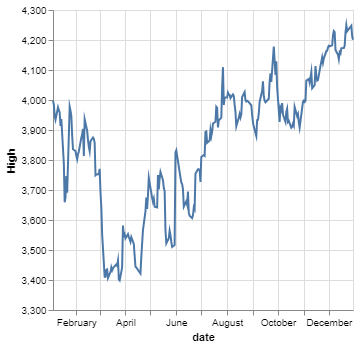
\includegraphics[width=.7\textwidth]{visualization (8).png}
\end{center}

To apply a rolling transform on the representation, use the \textit{transform\_window} function. Here we average data over a week time.

\begin{minted}[bgcolor=bg, frame=lines, framesep=2mm]{python}
chart = (
    alt.Chart(prices)
    .mark_line()
    .transform_window(
        rolling_mean='mean(High)',
        frame=[-7, 0]
    )
    .encode(
        alt.Y('rolling_mean:Q').scale(zero=False),
        x='date:T'
    )
)

chart
\end{minted}

\begin{center}
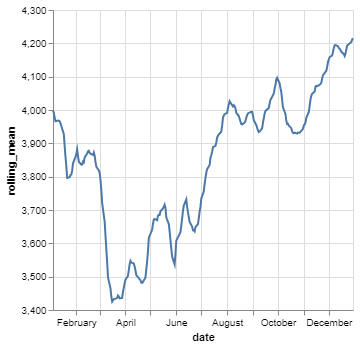
\includegraphics[width=.7\textwidth]{visualization (9).png}
\end{center}

To complete a Bollinger bands representation we add the standard deviation to the view.

\begin{minted}[bgcolor=bg, frame=lines, framesep=2mm]{python}
line  = (
    alt.Chart(prices)
    .mark_line()
    .transform_window(
        rolling_mean='mean(High)',
        frame=[-7, 0]
    )
    .encode(
        alt.Y('rolling_mean:Q').scale(zero=False),
        x='date:T'
    )
)

band = (
    alt.Chart(prices)
    .mark_area(
        opacity=0.25, color='gray'
    )
    .transform_window(
        rolling_mean='mean(High)',
        rolling_stdev='stdev(High)',
        frame=[-7, 0]
    )
    .transform_calculate(
        ci_upper=alt.datum.rolling_mean + alt.datum.rolling_stdev,
        ci_lower=alt.datum.rolling_mean - alt.datum.rolling_stdev
    )
    .encode(
        x='date:T',
        y='ci_lower:Q',
        y2='ci_upper:Q'
    )
)

line + band
\end{minted}

\begin{center}
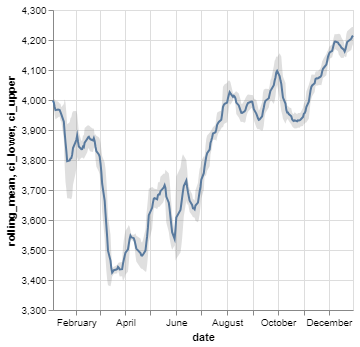
\includegraphics[width=.7\textwidth]{visualization (10).png}
\end{center}

\end{document}